\documentclass[a4paper, 12pt]{article}
\usepackage[T1]{fontenc}
\usepackage[utf8]{inputenc}

\usepackage[a4paper]{geometry}
\usepackage{titlesec}
\usepackage{amsmath}
\usepackage{amsfonts}
\usepackage{amsthm}
\usepackage{xcolor}
\usepackage{algorithm}
\usepackage{algorithmic}
\usepackage[bottom]{footmisc}
\usepackage[colorlinks=true, linkcolor=blue, citecolor=red, urlcolor=violet]{hyperref}
\usepackage{graphicx}
\usepackage{subcaption}
\usepackage{caption}


% FIGURES can be defined here and then used or directly defined within the text
\def\FigureOne{\centering\includegraphics[width=0.4\textwidth]{Figures/fig01.pdf}}

\def\FigureTwo{\centering\includegraphics[width=0.7\textwidth]{Figures/fig02.pdf}}
\def\FigureThree{\centering\includegraphics[width=0.4\textwidth]{Figures/fig03.pdf}}

\def\FigureFour{\centering\includegraphics[width=0.45\textwidth]{Figures/fig04.pdf}}

\def\FigureFive{\centering\includegraphics[width=0.8\textwidth]{Figures/fig05.pdf}}

\def\FigureSix{\centering\includegraphics[width=0.8\textwidth]{Figures/fig06.pdf}}

\def\FigureSeven{\centering\includegraphics[width=0.5\textwidth]{Figures/fig07.pdf}}

\def\FigureEight{\centering\includegraphics[width=0.6\textwidth]{Figures/fig08.pdf}}

\def\FigureNine{\centering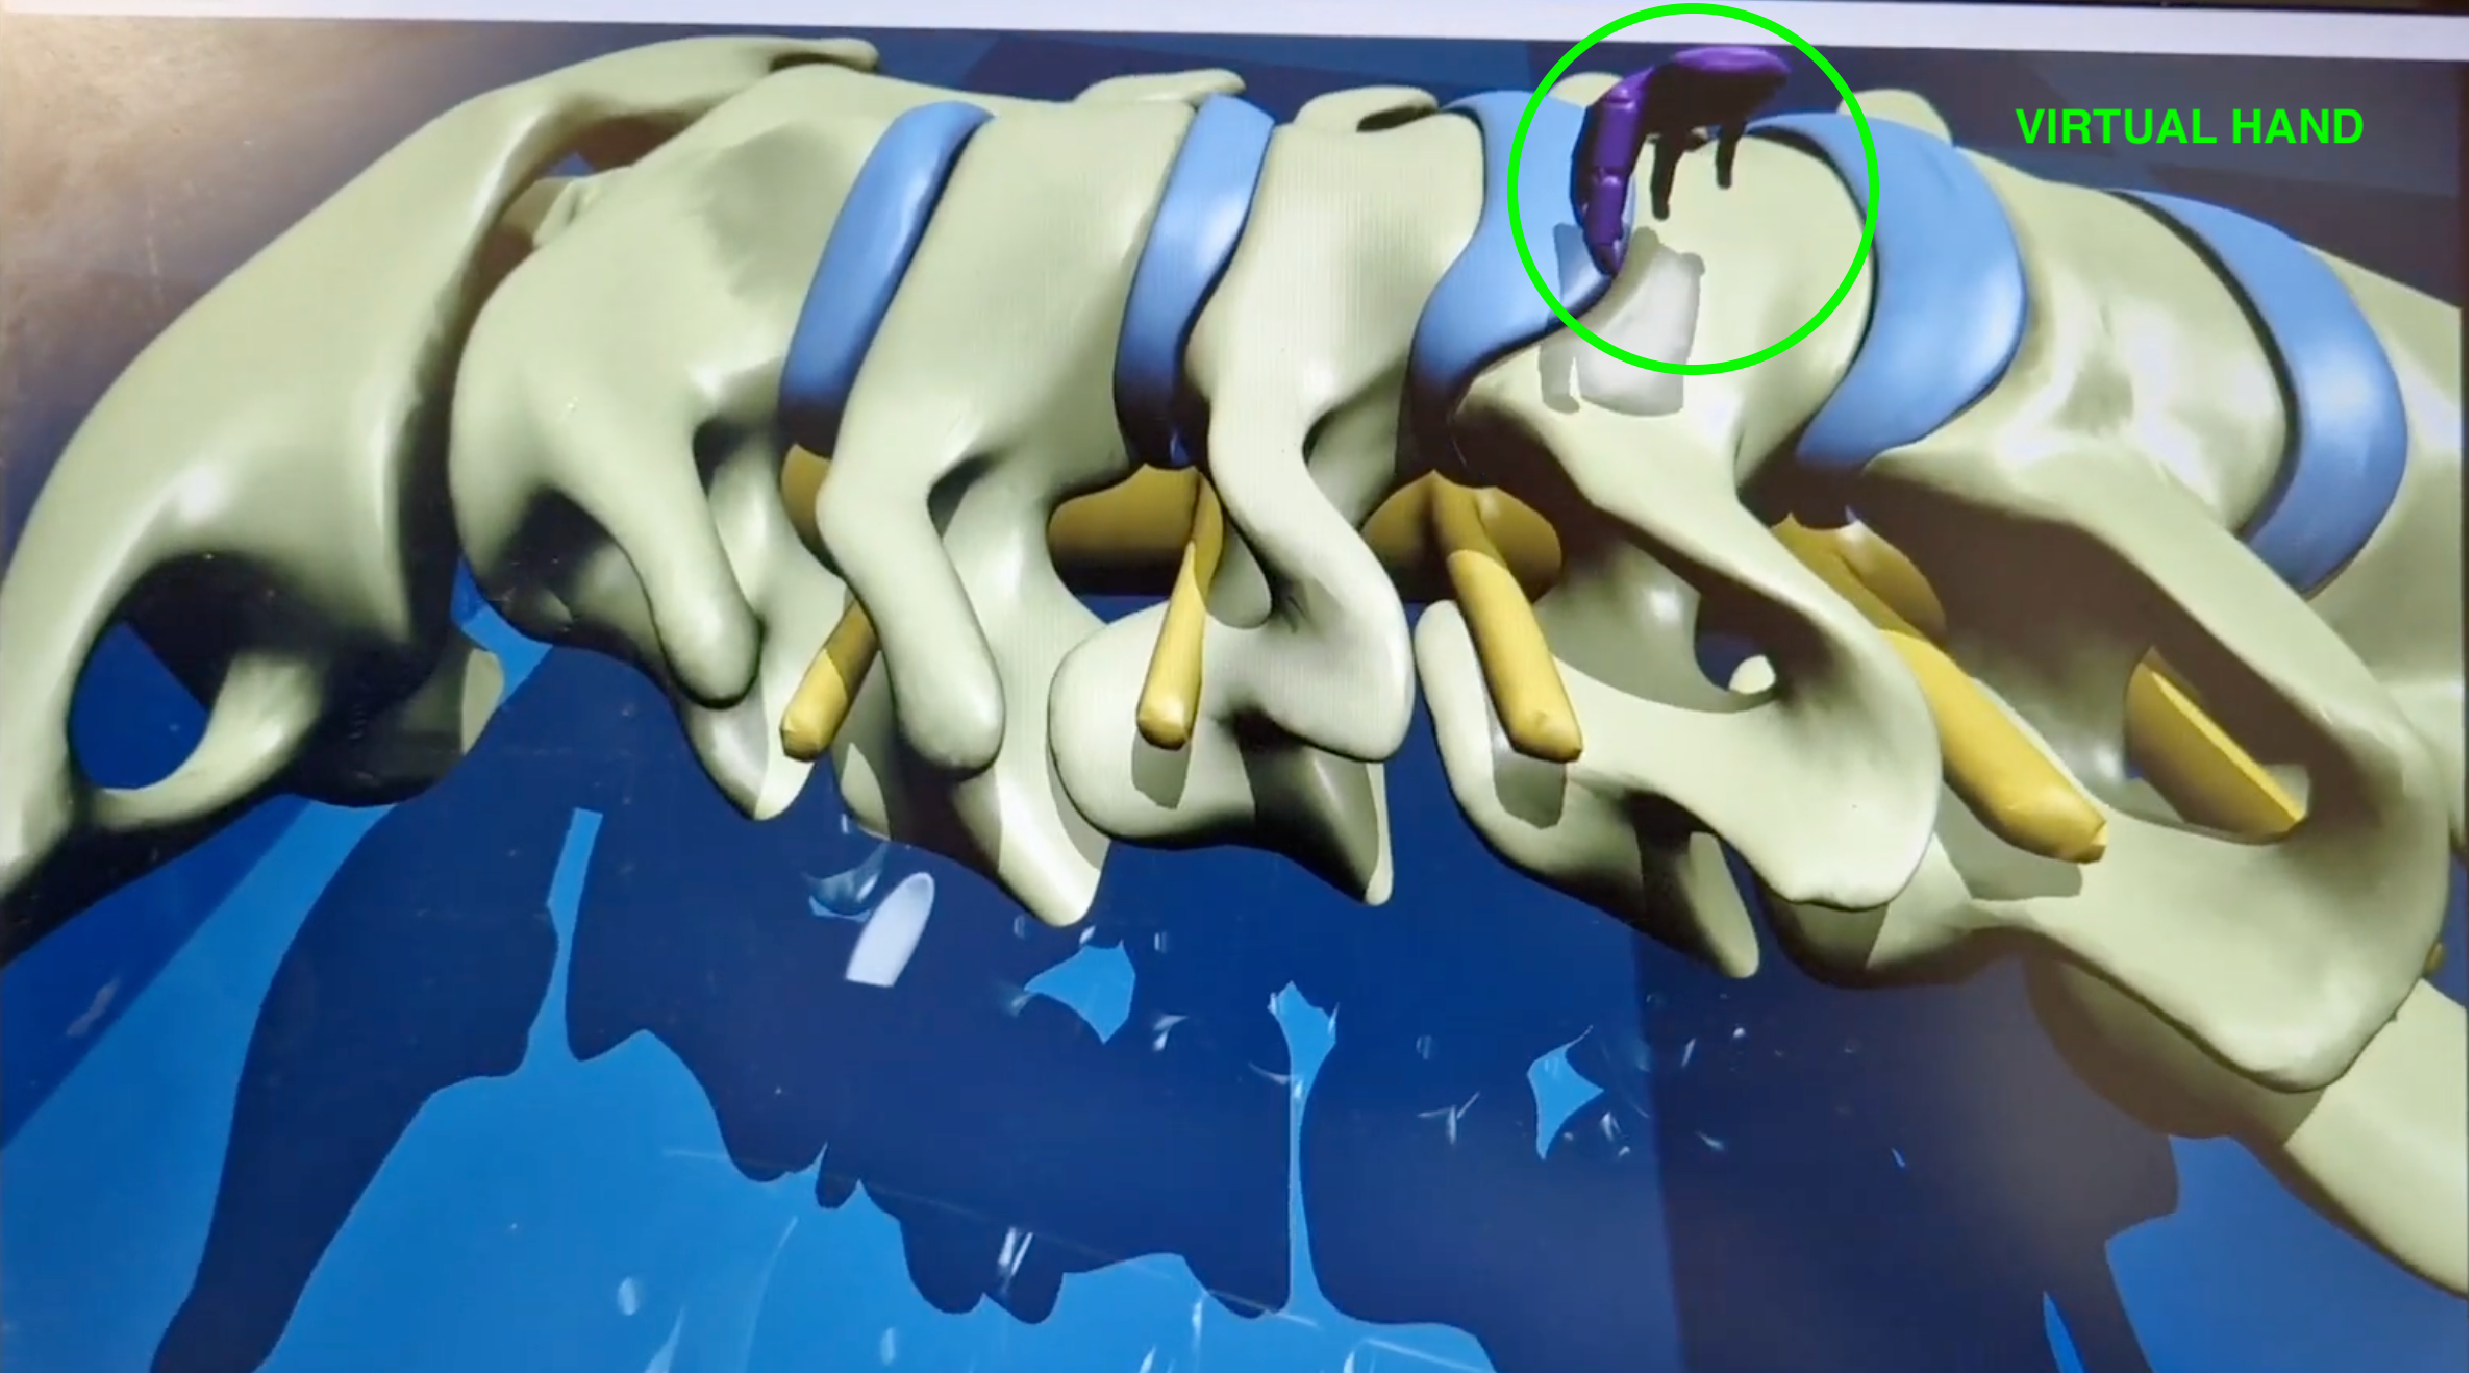
\includegraphics[width=0.8\textwidth]{Figures/fig09.pdf}}

\title{\textbf{Operational Report}}
\author{\textbf{Incarico di lavoro autonomo n. 27/2024} \\ \\ Matteo Scuderi - 1937090}
\date{}

\begin{document}

\maketitle
\section*{Purpose of the Collaboration}
The main purpose of this assignment is creating a "digital twin" for a surgery phantom, with the aim of integrating it in a digital VR simulation.\\
The said phantom is a 1:1 reproduction of the anatomical section bounded by the vertebrae C1 and C7, including all surrounding organs and tissues, such as muscles, blood vessels, esophagus and medulla. 
\begin{figure*}[h!]
    \FigureOne
    \caption*{\textbf{Figure I: } Spine Surgical Phantom in use}
    \label{fig:fig01}
\end{figure*}
\\This spine phantom is realized via additive manufacturing and therefore, a 3D model of each component was provided.
In the table below, a list of all components is reported, as well as some additional information (such as rigidity and color).
\begin{figure*}[h!]
    \FigureTwo
    \caption*{\textbf{Figure II: } Table of Phantom Components}
    \label{fig:fig02}
\end{figure*}
\clearpage
The simulation software chosen for the phantom's digital simulation is \\MuJoCo. This choice was agreed on with Prof. Vendittelli for three main reasons:
\begin{itemize}
    \item Realistic Simulation of contact forces (essential for surgical applications)
    \item Possibility of simulating deformable tissues/objects
    \item Experience of the writer in the use of the Software in medical applications.
\end{itemize}
 The followed workflow is shown below.
 \tableofcontents
 \section{Importing the 3D Model in MuJoCo}
 The preliminary step for simulation is importing the 3D model in the MuJoCo "scene" (i.e. the \textit{.xml} file).
 \\In order to better understand the issues with this procedure, a few MuJoCo requirements are stated below:
 \begin{enumerate}
     \item In MuJoCo, 3D models of each component must be imported as \textbf{single files} in a standard format (in this case, \textit{.stl}).
     \item Single files, or better \textit{meshes}, must have a vertex count below 100,000.
     \item For a smooth, bug-less simulation of contact forces, all meshes must be closed surfaces (in 3D-modeling lingo, they must be \textit{manifold}).
 \end{enumerate}
 As for point 1, the provided files were already separated component-wise. Unfortunately, some of them violate both Point 3 and/or Point 2.
 \\\\ For this reason, some modifications to the "incompatible" files were necessary. The 3D-modeling software \textbf{Blender} was used for this task.
 \subsection{Blender Modifications}
 Before discussing the chosen problem-solving strategy, a premise is necessary. The writer has no expertise in 3D-modeling and faced the said problem as a neophyte, having used Blender for the very first time. 
 \\Therefore, it is possible that the chosen strategy is not the most efficient, even though the result is still satisfactory, in the writer's opinion.
 \\\\The main tool used for making the \textit{.stl} files MuJoCo-compatible is Blender's built-in \textbf{\textit{remesh}} function.  This simple algorithm was used:\\
\begin{algorithm}[h!]
\caption{Remeshing for MuJoCo compatibility}
\begin{algorithmic}
    \STATE Import .stl files in Blender
    \FOR{each imported mesh}
        \IF{mesh is not "manifold"}
            \STATE Apply: Voxel Remesh
            \STATE Apply: Quad Remesh (4.000 Vertices)
        \ELSIF{\#Vertices > 100.000}
            \STATE Apply: Quad Remesh (4.000 Vertices)
        \ENDIF
    \ENDFOR
\STATE Export new meshes as single .stl files with scale 0.001 (for realistic dimensions)
\end{algorithmic}
\end{algorithm}
\begin{figure*}[h!]
    \FigureThree
    \caption*{\textbf{Figure III:} Blender Command for Remeshing}
    \label{fig:fig03}
\end{figure*} 
\\Applying this algorithm, all "non-manifold" meshes (i.e. not convex and closed) are firstly "decomposed" in voxels (3D pixels). After that, the object's surface is \textit{remeshed} with a Vertex count of 4.000, which reduces the file dimensionality (and consequently, the mesh quality) in order to make it MuJoCo-compatible. This last step is necessary for all \textit{.stl} files that violate Point 2 (vertex count above 100,000).
\\It is possible to choose a different balance between mesh quality and dimensionality, remeshing the files with an higher vertex count (as long as Point 2 is not violated).
\\\\After this process, all files can be imported in the MuJoCo scene (practically, in the \textit{.xml} file) using a command of this type:\\\\
$<geom\ name="name\_of\_component"\ mesh="path\_to\_mesh\_stl\_file"/>$
\subsection{Creation of the .xml file}
As previously mentioned, the scene's "topology" is created via an \textit{.xml} file. For generating this file, some additional python scripts were created.
\\\\Starting from a very "basic scene" (in which only some parameters are specified, but no objects are present), the script creates a new file and adds all the phantom's element with a hierarchical structure (parent-children). 
\\\\The \textit{.xml} file can be manually modified after its creation, adding or modifying both objects and parameters. However, the python script automates an otherwise tedious operation which is calculating the geometries' position in the scene.
\clearpage
\section{Building MuJoCo Scene}
In the implementation of the MuJoCo scene, three main key-points were considered: \textbf{computational demand, "user-friendliness" and realism}. All implementative choices were made to find a balance between the three. In particular sacrificing the latter often translates in an improvement of the other two key-points. Let's analyze these choices step by step,  so to reconstruct the "backbone" of the MuJoCo scene.
\subsection{CHOICE 1: Interactive Elements in the scene}
As the real surgical phantom includes a lot of flexible elements - such as muscles - its digital counterpart has to deal with some computational limitations. The hardware used for simulation struggles to run smoothly in presence of too many deformable objects, as their computational demand is elevated. For this reason, it was chosen to limit the interactibility of the scene to the  spine, as it will be the interested area in surgery. On the contrary, every other organ and tissue present is only a "background element" when the surgery is performed and their simulation is not as essential.
\\\\For this reason, \textbf{the main focus of this work was to replicate realistic spine movement} that matched the physical phantom's counterpart.

\subsection{CHOICE 2: Python Simulation vs Built-in MuJoCo Simulation}
MuJoCo's physics engine has some "primitives" that are common to most simulation Software (such as joints, actuators exc.). In particular, \textbf{joints} in MuJoCo assign to each object a certain number of \textbf{Degrees of Freedom} (from now on, \textbf{DOFs}). These DOFs define how the body can move in the scene - for instance, hinge joints define rotational motio around the joint's axis. A body with no DOFs is otherwise fixed in space and can't move even if forced.
\\\\ With this in mind, the challenge was \textbf{creating a "joint pattern" for the spine that would replicate the motion of interest in surgery}, while keeping in mind the three key-points previously defined. 
\\\\A first simplification was made and the spine was considered as a planar vibrating string. Of course, we would need a "discrete" version of the otherwise continuous and infinite-dimensional model, whereas we only have a certain number of vertebrae and discs that move according to this motion. In this scenario, the "nodes" are represented by the vertebrae C1 and C7 respectively, which in the phantom are attached to the structural frame and therefore fixed.
\begin{figure*}[h!]
    \FigureFour
    \caption*{\textbf{Figure IV:} Vibrating String Simplification}
    \label{fig:fig04}
\end{figure*} 
\\
With this premise we can face the main choice made so far: choosing between a Python-driven simulation or a built-in simulation.
\\
Let's suppose we've placed our joints in a certain way (i.e. assigned the DOFs that define the spine movement). We can now proceed in two ways. 
\begin{enumerate}
    \item \textbf{External (Python) Script:}\\
    Place actuators (for instance velocity/position controlled motors) and assign the joints' velocities/positions calculated as a solution of the vibrating string equation. This action must be performed in real-time with an external script (e.g. Python script) and is computationally demanding, especially if the phantom is inserted in a larger scene with other interactions to be simulated.\\
    Moreover, this choice hides some compatibility issues from the MuJoCo-Python integration. For example, on MacOS the Python script must be run through a plug-in called \textit{mjpython}, which however often crashed due to faulty implementation. As a result, any Mac owner would not be able to start the simulation due to compatibility issues. 
    \item \textbf{MuJoCo built-in Simulation:}\\
    In this case, the simulation runs natively in the MuJoCo application. This means that it can be run virtually on any computer, as the computational demand is much lower and there are no compatibility issues.
    Moreover, it can be easily integrated in a bigger scene, as there's no external code that might generate conflicts.
    On the down side, the built-in MuJoCo engine only allows direct assignment of \textbf{constant} actuator's references. Therefore, the "vibrating string" dynamics can't be assigned. Instead, one must build, using the engine's primitives, an interconnection between the spine elements that behaves as close as possible to the said string. 
    \\ In this way, the spine will deform when interacted with, but all the computations will be held in real-time by the physics engine only - again, reducing computational expense drastically.
\end{enumerate}
The best option with respect to the three key-points was found to be the latter.
\subsection{Choice 3: Joints' Configuration and Interconnections}
To recap, the problem at this point was to \textbf{find a configuration of MuJoCo primitives that approximate the string-like behavior of the spine.}
\\ At first, it was considered to use prismatic joints -one for each vertebra and each disc- to emulate the sting-like behavior. However, this choice produced a "staircase-like" motion that wasn't satisfactory. A snapshot of such movement is shown below.
\begin{figure*}[h!]
    \FigureFive
    \caption*{\textbf{Figure V:} Staircase-like movement}
    \label{fig:fig05}
\end{figure*}
\\In red, we can see the approximated shape that is created by interacting with the spine, while the blue arrows represent the prismatic joints' direction of motion. This staircase-like movement is even more evident in simulation, as the spine dynamically rearranges but maintains the same kind of squared pattern.
\\\\ To avoid this non realistic behavior, it was decided to use \textbf{a combination of hinge joints and tendons}. In fact, hinge joints are used to model each vertebra/disc rotation around the "string" normal axis. Of course, such joints are limited to allow only small-angle rotations, as for a real spine wouldn't allow great deformations without breaking. The tendons are added to "link" all the joints and merge all the single rotations into a smooth movement. In fact, tendons in MuJoCo are nothing but \textbf{global mobility constraints} imposed between the joints of interest. This translates into a much smoother and more realistic behavior, as shown below. The movement is much more arch-shaped and the joints' axes are shown as blue spikes.
\begin{figure*}[h!]
    \FigureSix
    \caption*{\textbf{Figure VI:} Arch-shaped movements}
    \label{fig:fig06}
\end{figure*}
\subsection{Choice 4: Parameters}
At this point, the scene has a well defined structure that allows quite realistic simulation of the spine's string-like behavior. What can be done to improve the final version of the scene is to \textbf{tune the physical parameters} of the spine elements.
\\\\This can be done directly on the \textit{.xml} file using MuJoCo's built-in physics engine's parameters.
In particular, we can adjust (to make a few examples), the components' masses and inertia, as well as joints' elasticity, damping and limits.
\\\\
However, notice that \textbf{several tuning paradigms can be made depending on the application of use for this scene}. For purely didactical purposes, one could accentuate the spine's mobility in order to allow larger curvature (which wouldn't be allowed, for instance, in a surgery). This can be easily obtained by imposing larger joint limits and longer tendons.
\\On the contrary, one could reduce spine mobility and adjust joint damping/elasticity to try to match the physical phantom's properties. This would instead be the right choice for creating a digital twin. 
\\\\The "parameter tuning" done by the writer was in the direction of \textbf{compromise between the two possible applications}. On one hand, accentuate a bit the spine's mobility so to show the correct behavior and make the simulation enjoyable by non-experts. On the other, not exaggerate such mobility and add elasticity/damping to make it more similar to the physical phantom.
\\\\ 
Notice that moving the tuning paradigm towards the didactical purpose can be easily obtained via some in-simulation trial and error, which can be done using the MuJoCo application only. \\Vice-versa, moving towards the digital twin requires to work in a virtual reality environment (possibly, with some haptic glove) and in close contact with the physical phantom. In fact, for this purpose one must try to match the real-life feeling of "deformation" and "hardness" of the physical spine with the feeling rendered by MuJoCo and the haptic glove. To have a realistic interaction between the spine and the user's hand, it's necessary to track its movements in the scene, hence one must use a VR environment to simulate the scene.
\\\\
Before discussing the VR integration of the scene, let's briefly discuss the final version of the simulation (which again can run on the MuJoCo application with no external script).

\section{Final MuJoCo Scene}
The final scene involves all the elements that compose the physical phantom. 
In particular, the writer decided to split the components into five groups [1,2,3,4,5], since each group can be enabled/disabled by just pressing one button. As a result, one can remove from the scene some "layers" to better visualize the inner ones.
\begin{figure*}[h!]
    \FigureSeven
    \caption*{\textbf{Figure VI:} Group enable/disable}
    \label{fig:fig07}
\end{figure*}
\subsubsection{Group 1: Frame}
This group only contains the structural elements of the physical phantom. Therefore, these components would not be present in a real human patient, but are strictly necessary to hold the physical phantom in place.
\subsubsection{Group 2: Various}
This group is the most variegated one as it includes organs (such as the esophagus and thyroid), membranes, muscles and nerves.
As for the muscles, it includes all those that "surround" the human throat and support the spine. In the future, it would be interesting to make them deformable (once again, impossible as for now due to hardware limitations and computational overload).
 They're grouped together with other "background" organs as they're not of interest for spinal surgery and MuJoCo only allows 6 total groups for its scenes.
\subsubsection{Group 3: Veins}
This group is made of arteries and veins. They all could be elements of interest in a surgery, as damaging a blood vessel is something to avoid at all costs. However, at the moment they're all left as non-interactible objects. A relatively easy task to add would be to implement some kind of contact detection, whereas "damage" and perforation simulation would be a much more complicated problem.
\subsubsection{Group 4: Medulla}
This group is only made by two objects: inner and outer medulla. Since it's an element of interest for spinal surgery, it can be made interactible in a similar manner as for the blood vessels. However, for complicated problems such as needle insertion, a lot more of study on the Software must be done.
Notice also that \textbf{medulla is not deformable}, hence it doesn't match the spine deformation. For small spine "arches" this is barely an issue, but for greater mobility it can disrupt the authenticity of the simulation.
\subsubsection{Group 5: Spine}
Finally, the last group is made by vertebrae and discs. As previously discussed, each element possesses a rotational DOF and is linked to the adjacent vertebra/disc by a tendon. The resulting structure behaves like a vibrating string fixed on both ends. In particular, the first and last vertebrae (C1, C7) are fixed in place using a \textbf{welding constraint} (MuJoCo built in functionality).
\\\\In the next page, images of these groups are reported.
\clearpage
\begin{figure*}[h!]{}\
\centering
    \begin{subfigure}[t]{0.5\textwidth}
\includegraphics[width=\textwidth]{Figures/fig08a.pdf}
           \subcaption{\textbf{Group 1:} Frame}
           \label{fig:fig08a}
    \end{subfigure}
    \begin{subfigure}[t]{0.45\textwidth}
    \includegraphics[width=\textwidth]{Figures/fig08b.pdf}
           \subcaption{\textbf{Group 2:} Various}
           \label{fig:fig04b}
    \end{subfigure}
        \begin{subfigure}[t]{0.45\textwidth}
\includegraphics[width=\textwidth]{Figures/fig08c.pdf}
           \subcaption{\textbf{Group 3:} Veins}
           \label{fig:fig08c}
    \end{subfigure}
    \begin{subfigure}[t]{0.5\textwidth}
    \includegraphics[width=\textwidth]{Figures/fig08d.pdf}
           \subcaption{\textbf{Group 4:} Medulla}
           \label{fig:fig04d}
    \end{subfigure}
        \begin{subfigure}[t]{0.45\textwidth}
\includegraphics[width=\textwidth]{Figures/fig08e.pdf}
           \subcaption{\textbf{Group 5:} Spine}
           \label{fig:fig08e}
    \end{subfigure}
    \begin{subfigure}[t]{0.5\textwidth}
    \includegraphics[width=\textwidth]{Figures/fig08f.pdf}
           \subcaption{\textbf{Full Digital Phantom}}
           \label{fig:fig04f}
    \end{subfigure}
    \caption*{\textbf{Figure VIII:} Visualization in MuJoCo of the Digital Phanom}
    \label{fig:fig08}
   \end{figure*}
\clearpage
\section{VR and Haptic Glove Integration}
Taking advantage of the writer's previous work, it was relatively easy to add the digital phantom to a bigger scene. In particular, the phantom was inserted in a scene that integrated Virtual Reality (thanks to Oculus Rift S and openxr) and the WeArt Haptic glove. This allows to replicate the user's hand and fingers' movement on a virtual hand that's inserted in the VR simulation. Moreover, thanks to the haptic glove, the user perceives the contact forces with virtual objects on his fingertips.
\\\\Of course this kind of simulation can only run thanks to an external (Python) script that also handles all communications between the various devices and environments. It's clear that the computational power required is substantial and not all hardware can perform such operation. That's why the work done in simulating the spine using only MuJoCo primitives is important in order to not weigh down even more the computational load.
A snapshot of the integrated VR environment is shown below. 
\begin{figure*}[h!]
    \FigureNine
    \caption*{\textbf{Figure IX:} VR Integrated Simulation}
    \label{fig:fig09}
\end{figure*}
\\In this simulation, it was chosen to rescale the spine by a factor $10$x, for purely didactical purposes. The virtual hand can be seen near the top left corner and caused the deformation (arch) visible in the figure.
\clearpage
\section{Personal Considerations and Possible Further Developments}
The main challenge with this kind of technology is finding a balance between the three key-points (computational demand, "user-friendliness" and realism). The first one represents the biggest factor to take into account, as a non-smooth simulation disrupts the whole experience, especially for VR integrated experiences. I've tried to work with this idea in mind, often making compromises to keep the scene "light".
\\That's one of the reasons I discarded the idea of simulating the spine by solving differential equations and assigning joint references with an external Python script. However, this could still be a possibility, as long as one can make a good enough mathematical model. 
\\\\
The MuJoCo model can surely be improved depending on the use, but I believe it's a solid base for further developments. 
\\\\If the main goal is to create a digital twin for the physical phantom, then it is necessary to start working side by side with it and tune all the spine's parameters trying to match the phantom's behavior. This process will surely take time and will be mostly a matter of trial and error. With enough attempts, I'm confident that good results can be obtained.
\\\\If the final goal is creating a didactical tool instead, one can work with scaling the model (as in the VR experience created) and "exaggerate" spine mobility, as well as making more elements interactible.
\\\\An interesting idea could be to integrate neural networks in the simulation of deformable objects (as shown by Doctor De Santis). One could start for instance from the medulla, which at the moment doesn't deform with the spine but is instead static. It's surely an easier task than simulating deformable closed surfaces (such as kidneys) as medulla could be approximated to a vibrating string as well. 
\\I'm not sure how much work is necessary to do such thing, but it could be worth investigating.
\\\\In the hypothesis of having a surgeon trainee operating on the physical phantom, instead, one could use a camera and computer vision techniques to reconstruct the phantom spine pose, and then assign directly the joint references from that information. This would eliminate the need for simulating the "vibrating cord" dynamics and allow for a 1 on 1 matching of the exact pose of each vertebra/disc. However, this is a case of application for which the simulation is used as an additional tool to the "in-real-world" training and wouldn't work for "virtual" training.
\end{document}